%-------------------------------------------------------------
% 导言区
\documentclass[dvipsnames]{beamer}
\usepackage[utf8]{inputenc}
\usepackage{hyperref}
\usepackage[T1]{fontenc}
\usepackage{chemformula}

\usepackage{listings}

\usepackage{latexsym,multicol,booktabs}
%\usepackage[dvipsnames]{xcolor}
%\usepackage{calligra}
\usepackage{amsmath,amssymb,siunitx}
\usepackage{bbm}
%\usepackage{amsmath,multicol}
%\usepackage{BOONDOX-cal}
\usepackage{bm}		%   数学公式宏包
\usepackage{graphicx,pstricks,stackengine}      
\usepackage{subcaption}
\usepackage{comment}

\lstset{
  basicstyle=\fontsize{8}{13}\selectfont\ttfamily
}

%   个人信息
\author{Raffaele Ancarola}
\title{Spatial variability addressed with random fields and Bayesian inversion}
\institute{Geomod, Stéphane Commend}    
\date{\today}

\logo{
\includegraphics[height=0.3cm]{images/geomod.jpg}\hspace*{0.15cm}}

%   设置主题文件    后缀名为.sty的文件是一个主题文件,初学者不要修改sty文件
\usepackage{SCU}



%   defs 特殊字体
\def\cmd#1{\texttt{\color{red}\footnotesize $\backslash$#1}}
\def\env#1{\texttt{\color{blue}\footnotesize #1}}


%   简化定理命令
\newtheorem{thm}{Theorem}[theorem]

%\newcommand{\hbar}{\mathchar'26\mkern-9mu h}
\newcommand{\diff}[2]{\frac{\partial #1}{\partial #2}}
\newcommand{\ddiffx}[1]{\frac{\partial^2 }{\partial #1^2}}
\newcommand{\ddiff}[2]{\frac{\partial^2 #1}{\partial #2^2}}
\newcommand{\ddiffd}[3]{\frac{\partial^2 #1}{\partial #2 \partial #3}}
%—-------------------------------------------------------------
% 正文区

\begin{document}

	% 封面
	\begin{frame}
		\titlepage
	\end{frame}
	
	% 目录
	%\begin{frame}
	%	\tableofcontents[sectionstyle=show,subsectionstyle=show/shaded/hide,subsubsectionstyle=show/shaded/hide]
	%\end{frame}
		
	
	%—------------------------------------------------------
	% 正文
		
	\section{Random fields and Bayesian inversion}
	
	\begin{frame}{What's a Random field?}
	\begin{block}{How it's defined?}
	Mean $\mu(\vec{x})$, variance $\sigma(\vec{x})$ and correlation function $C(\vec{x}, \vec{y})$.
	\end{block}
	
	\begin{figure}
	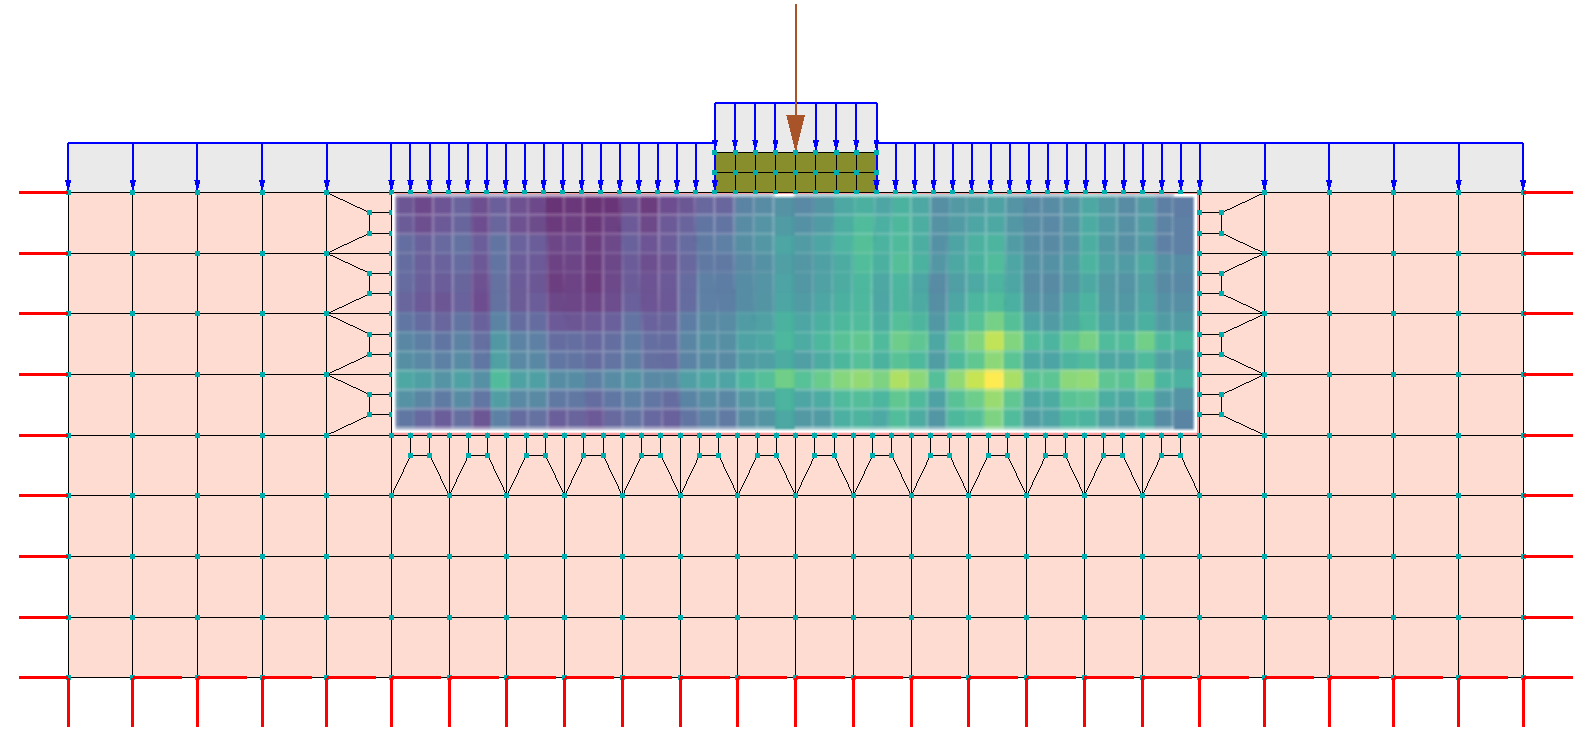
\includegraphics[width=0.8\textwidth]{images/rf_view.png}
	\caption{Sample of random field projected into a finite element mesh.}
	\end{figure}
	\end{frame}
	
	\begin{frame}{What's useful for?}
	\begin{columns}
	\begin{column}{0.5\textwidth}
	\begin{block}{Uncertainty quantification}
	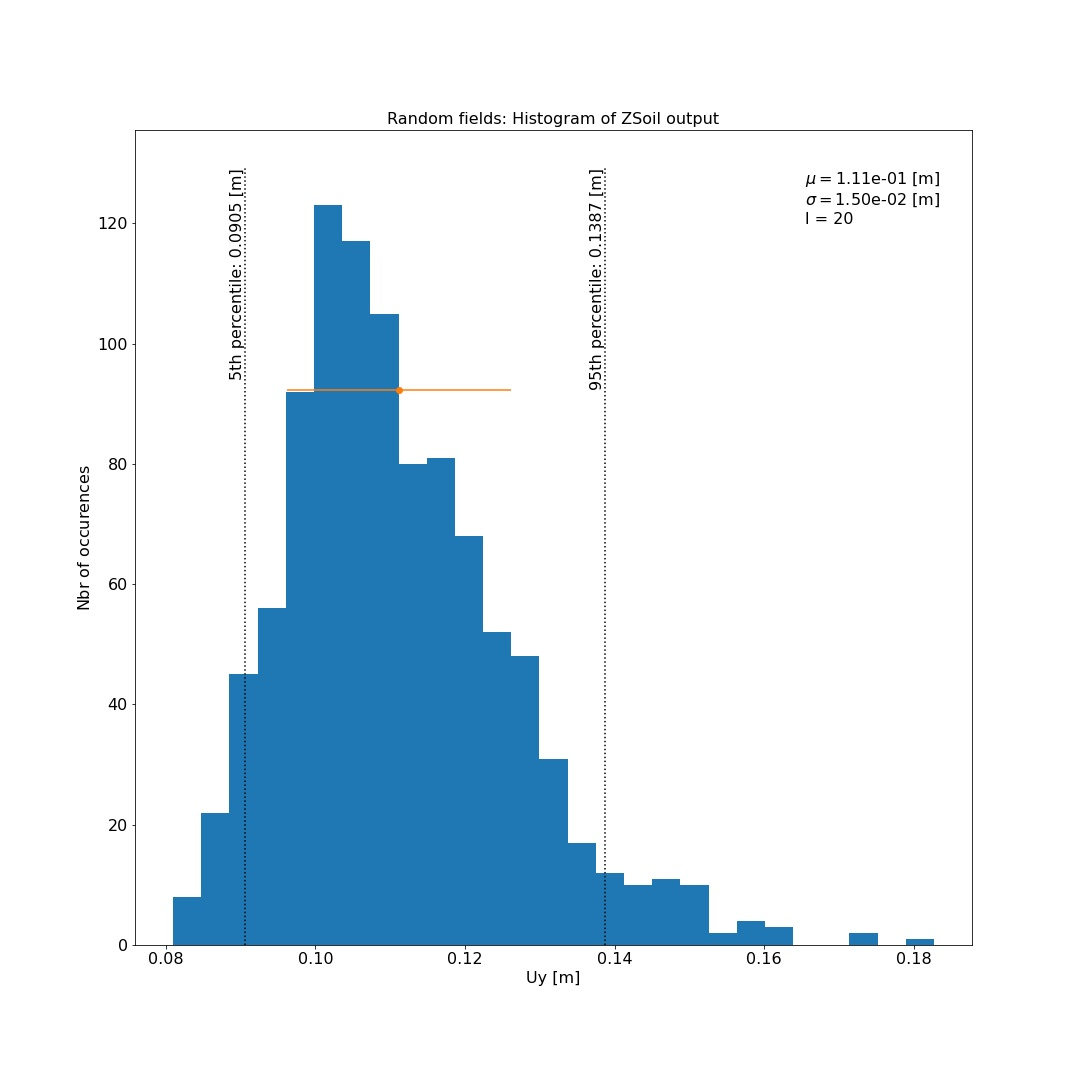
\includegraphics[width=\textwidth]{images/rf_hist.jpg}
	\end{block}
	\end{column}
	\begin{column}{0.5\textwidth}
	\begin{block}{Spatial variability}
	\vspace{0.5cm}
	
\includegraphics[width=\textwidth]{images/gradient.jpg}
	\end{block}
	
	\end{column}
	\end{columns}
	\alert{Keywords: REALISM and ACCURACY!}
	\end{frame}
	
	\begin{frame}{Exponential decay correlation}
	\begin{figure}
	\begin{subfigure}{.48\textwidth}
	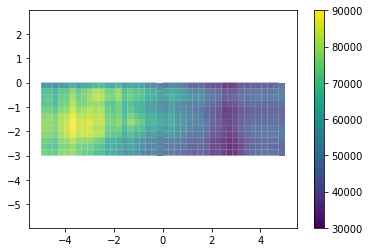
\includegraphics[width=\textwidth]{images/correlation_20.png}
	\caption{$l_x = 20$}
	\end{subfigure}
	\begin{subfigure}{.48\textwidth}
	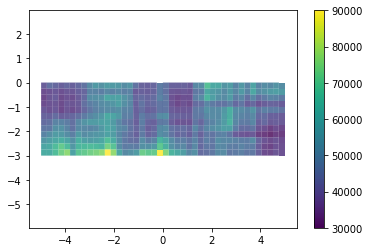
\includegraphics[width=\textwidth]{images/correlation_2.png}
	\caption{$l_x = 2$}
	\end{subfigure}
	\end{figure}
	\alert{This is still user defined.}
	\end{frame}
	
	\begin{frame}{What's meant by Bayesian inversion?}
	\begin{block}{Bayes theorem}
	\[ p(x| Y = y) = \frac{p(y | X = x) p(x)}{p(y)} \propto \mathcal{L}(x; y) p(x)\]
	\end{block}
	\begin{columns}
	\begin{column}{.5\textwidth}
	\begin{block}{Measurements $Y$: real data}
	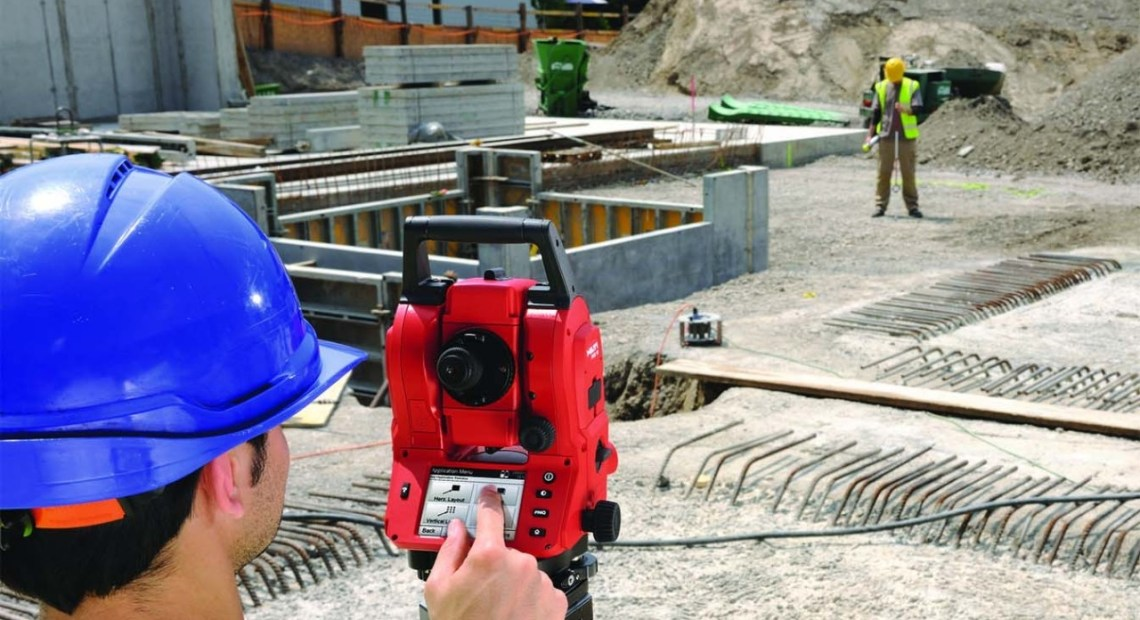
\includegraphics[width=\textwidth]{images/1111measure.jpg}
	\end{block}
	\end{column}
	\begin{column}{.5\textwidth}
	\begin{block}{Parameter update: posterior}
	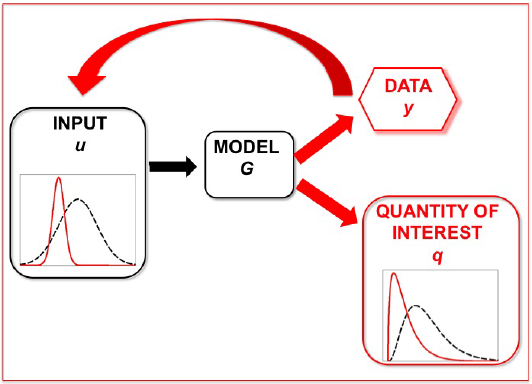
\includegraphics[width=\textwidth]{images/bayes_inv.png}
	\end{block}
	\end{column}
	\end{columns}
	\end{frame}
	
	\begin{frame}{Computational methods for Bayesian inversion}
	\begin{columns}
	\begin{column}{.5\textwidth}
	\begin{block}{Sample based}
	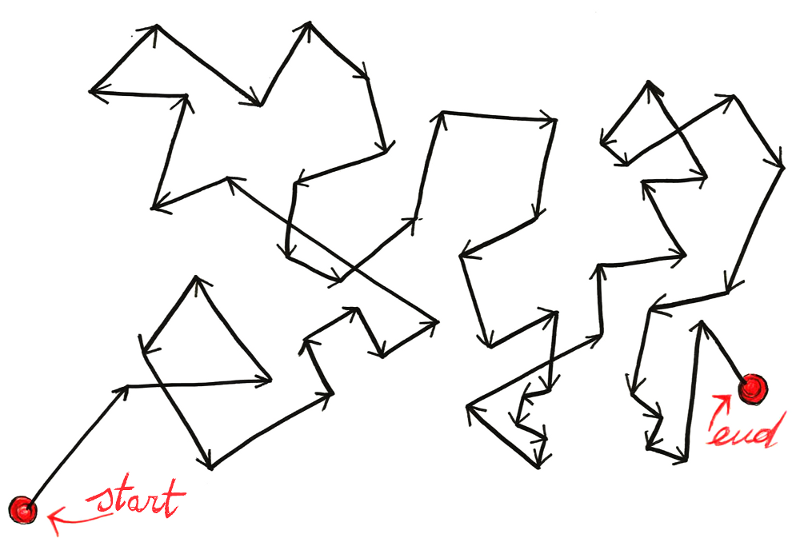
\includegraphics[width=\textwidth]{images/random_walk.png}
	\begin{itemize}
	\item Monte Carlo Markov Chain (MCMC)
	\end{itemize}
	\end{block}
	\end{column}
	\begin{column}{.5\textwidth}
	\begin{block}{Parametric}
		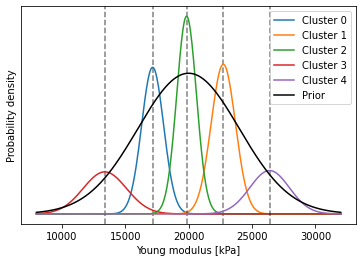
\includegraphics[width=\textwidth]{graphs/prior/K=5_all_details.png}
	%\begin{align*}
	%& \mathbb{E}[X_{post}] = \dots \\
	%& \texttt{var}(X_{post}) = \dots 
	%\end{align*}
	\begin{itemize}
	\item Gaussian mixtures (GLLiM)
	\item Likelihood expansions (SLE)
	\end{itemize}
	\end{block}
	\end{column}
	\end{columns}
	\end{frame}
	
	
	
	\section{Inversion of 1D Random field: Simply supported beam}
	
	\begin{frame}{Same problem, different approaches}
	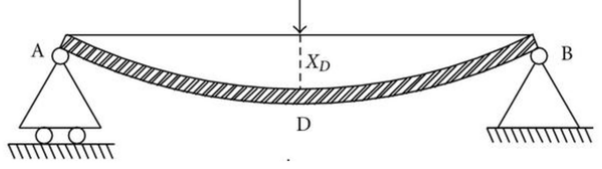
\includegraphics[width=\textwidth]{simply_supported_beam.png}
	\begin{columns}
	\begin{column}{.5\textwidth}
	\begin{block}{Flexibility: $\mathcal{M}(F) \propto F$}
	\[\ddiff{U_y}{x} = \frac{F(x)M(x)}{P} \]
	\end{block}
	\end{column}
	\begin{column}{.5\textwidth}
	\begin{block}{Young modulus: $\mathcal{M}(E) \propto 1/E$}
	\[\ddiff{U_y}{x} =  \frac{M(x)}{E(x)I}\]
	\end{block}
	\end{column}
	\end{columns}
	\end{frame}
	
	\begin{frame}{ZSoil finite element equivalent}
	\begin{figure}
	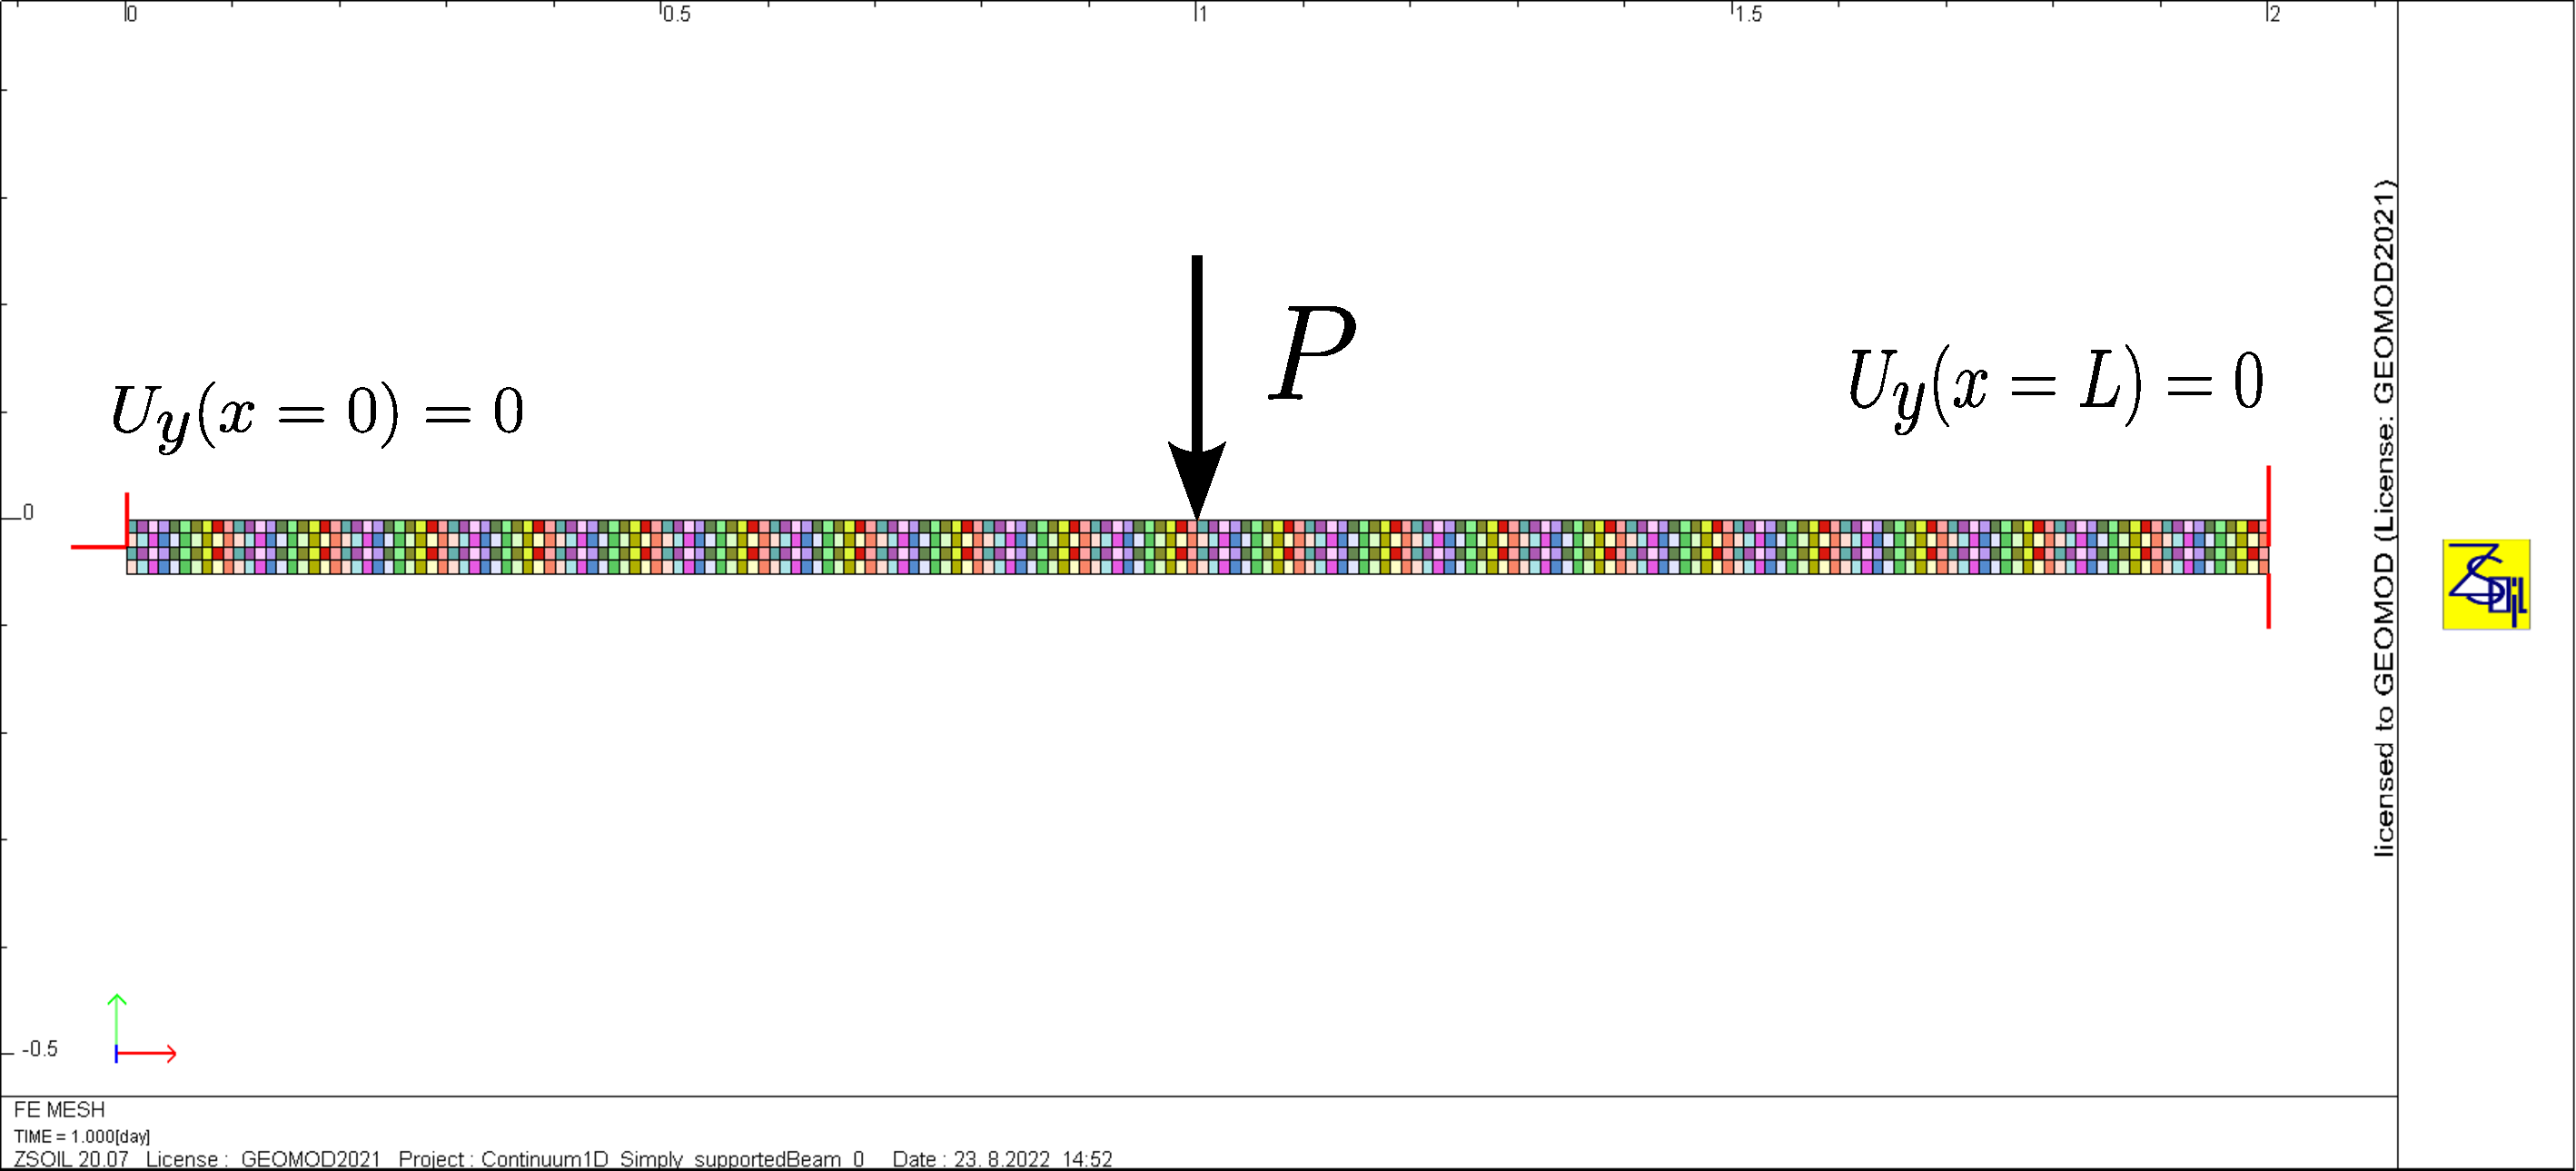
\includegraphics[width=\textwidth]{images/zsoil_ssb.pdf}
	\caption{Finite element \texttt{ZSoil} pre-processing model of simply supported beam.}
	\end{figure}
	\end{frame}
	
	\begin{frame}{Deflection prior and measurements}
	\centering
	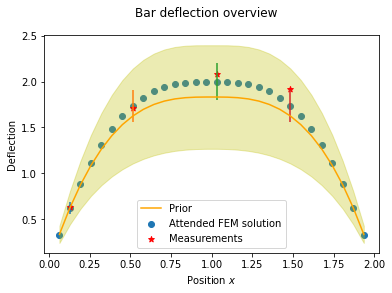
\includegraphics[width=0.8\textwidth]{setup.png}
	\end{frame}
	
	\begin{frame}{How to correct it?}
	\centering
	
\includegraphics[width=\textwidth]{correct.png}
	\vspace{1cm}
	\begin{center}
		{\Huge \emph {\textrm{With ~Bayesian ~inversion!}}}
		\end{center}
	\end{frame}
	
	\begin{frame}{Bayesian inversion of Flexibility $F$ (Linear)}
	\centering
	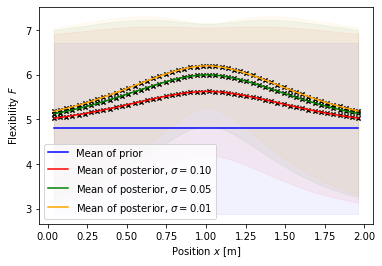
\includegraphics[width=\textwidth]{graphs/linear/flex_mapping.png}
	\end{frame}
	
	\begin{frame}{Bayesian inversion of Young modulus $E$ (Inverse)}
	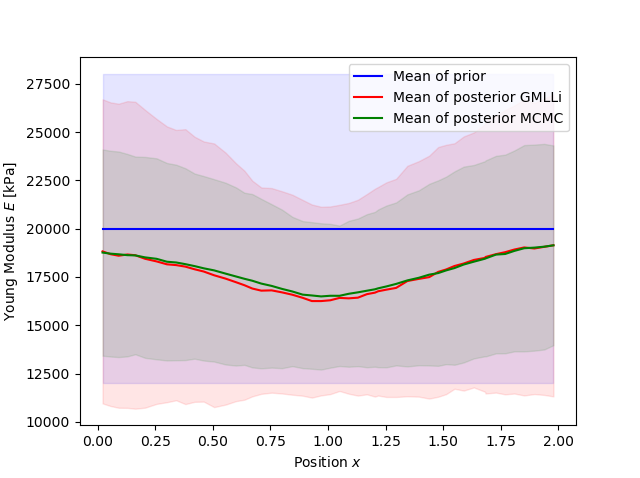
\includegraphics[width=\textwidth, height=0.9\textheight]{graphs/rf_E/young_map.png}
	\end{frame}
	
	\begin{frame}{Prior and posterior distributions form}
	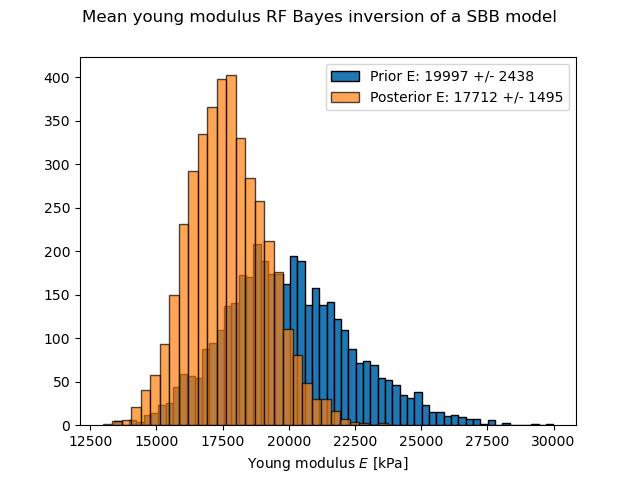
\includegraphics[width=\textwidth, height=0.9\textheight]{graphs/rf_E/young_modulus_hist.png}
	\end{frame}
	
	\begin{frame}{More complex systems: \texttt{ZSoil} and \texttt{ZSwalls} models}
	%TODO: add classes
	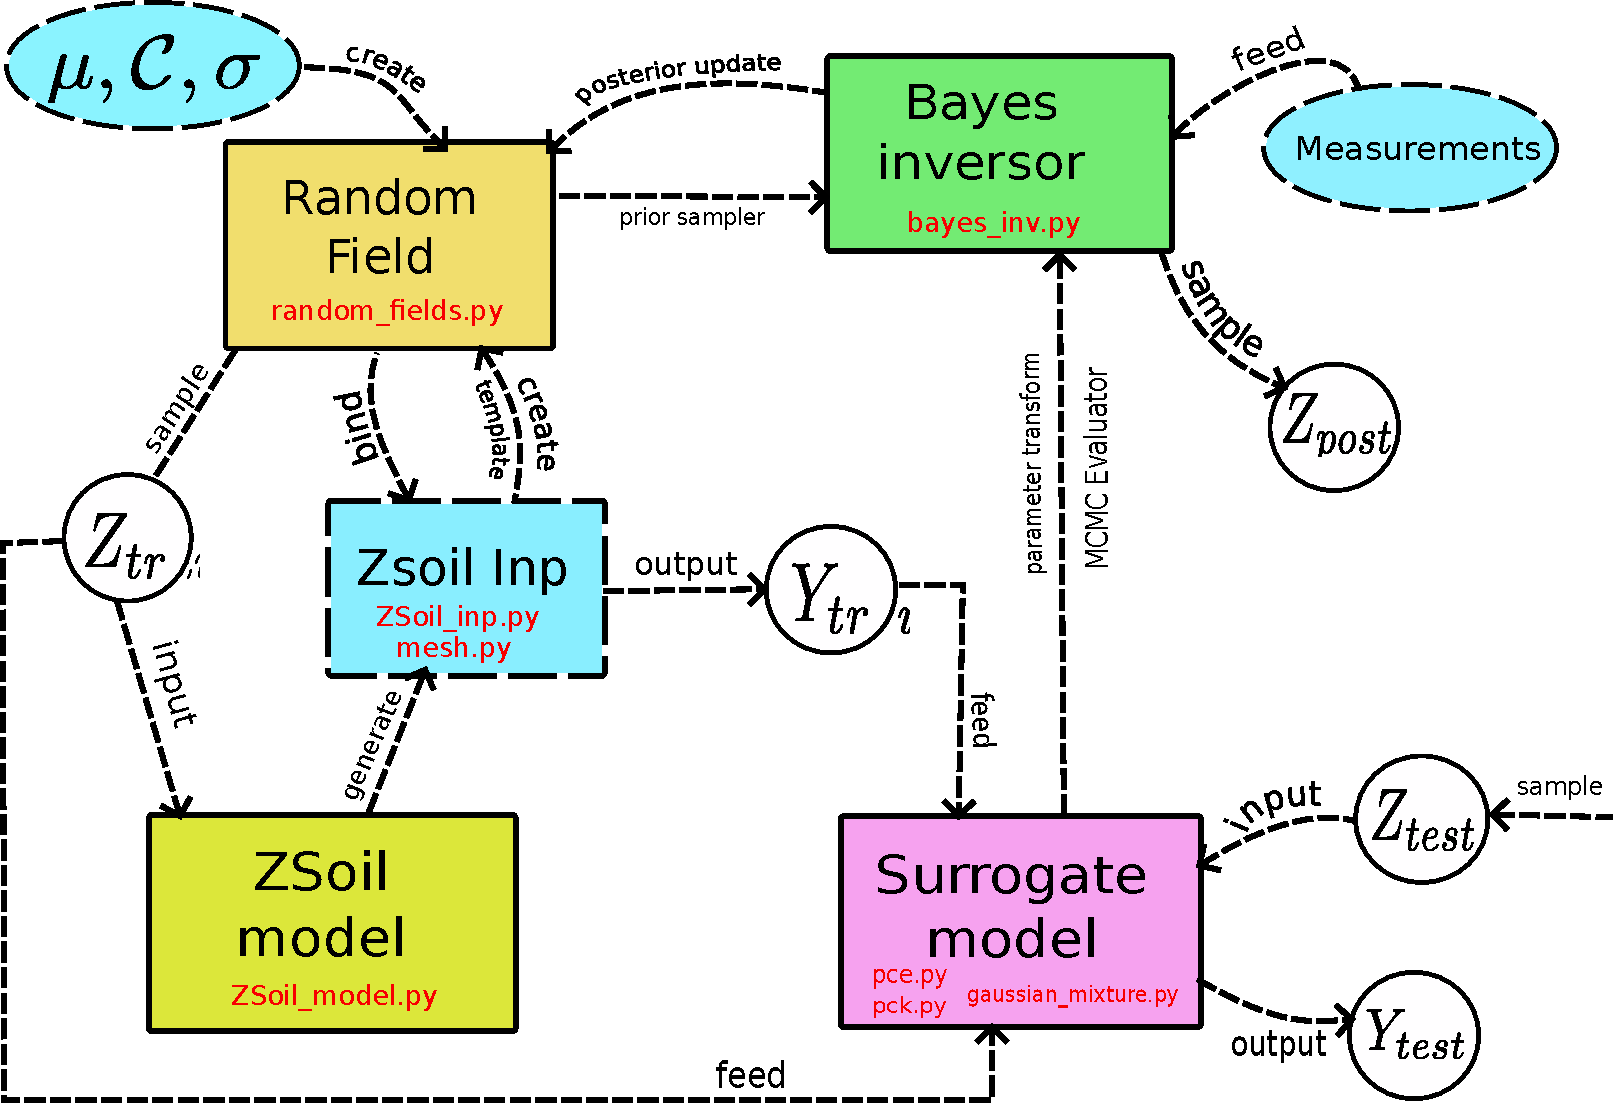
\includegraphics[width=\textwidth]{workflow.pdf}
	\end{frame}
	
	\begin{comment}
	\section{Some Bayesian inversion methods}
	
	\begin{frame}{Sample based: Monte Carlo Markov Chain (MCMC)}
	\begin{columns}
	\begin{column}{.5\textwidth}
	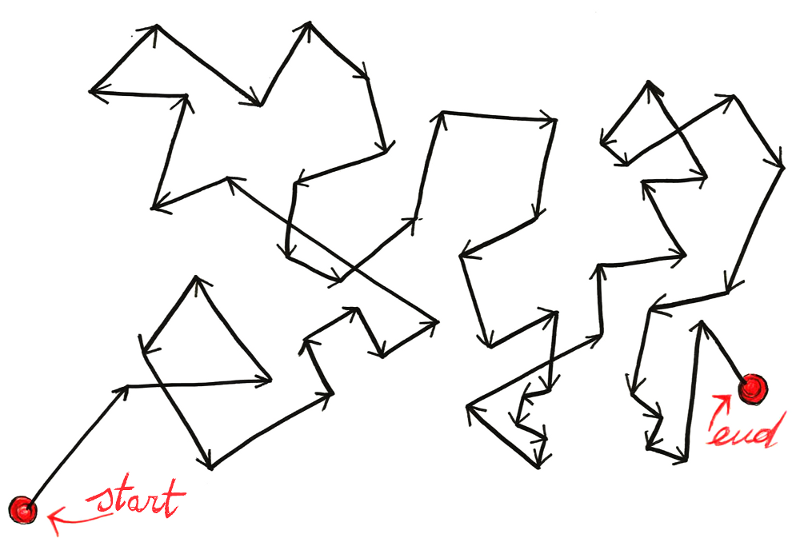
\includegraphics[width=\textwidth]{images/random_walk.png}
	\end{column}
	\begin{column}{.5\textwidth}
	\begin{itemize}
	\item Evolve chains to a likely state.
	\item Obtain samples.
	\end{itemize}
	\end{column}
	\end{columns}
	
	\begin{block}{Metropolis algorithm}
	\begin{itemize}
	\item Random walk: move $x^{(t)}$ to $x^{(*)}$ randomly.
	\item Accept $x^{(*)}$ with probability $\min\left(1, \frac{p(x^{(*)} | Y)}{p(x^{(t)} | Y)} \right)$.
	\item Repeat until convergence.
	\end{itemize}
	\end{block}
	\end{frame}
	
	
	\begin{frame}{GLLiM: Gaussian Locally Linear Mapping}
	\begin{columns}
	\begin{column}{.5\textwidth}
	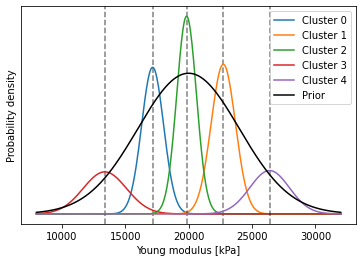
\includegraphics[width=\textwidth]{graphs/prior/K=5_all_details.png}
	\end{column}
	\begin{column}{.5\textwidth}
	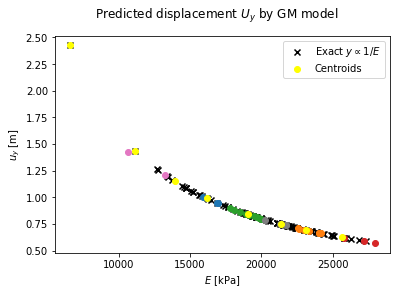
\includegraphics[width=\textwidth]{graphs/E_single/bayes_inversion_model_fit_view.png}
	\end{column}
	\end{columns}
	\begin{itemize}
	\item Mixture of $K$ gaussians.
	\item Approximate the prior distribution and the model at once.
	\item Deduce conditional properties (mean, variance, $\dots$).
	\end{itemize}
	\end{frame}
	
	\begin{frame}{Comparison: which is better?}
	\begin{columns}
	\begin{column}{.5\textwidth}
	\begin{block}{MCMC}
	
	Pros:
	\begin{itemize}
	\item Reliable if well set up.
	\item Obtain a lot of samples.
	\end{itemize}
	Drawbacks:
	\begin{itemize}
	\item Too many steps.
	\item Many model evaluations: needs \texttt{PCE}. 
	\end{itemize}
	
	\end{block}
	\end{column}
	\begin{column}{.5\textwidth}
	\begin{block}{GLLiM}
	
	Pros:
	\begin{itemize}
	\item Fast
	\end{itemize}
	Drawbacks:
	\begin{itemize}
	\item Lacks of accuracy.
	\item Too many training points for the model.
	\end{itemize}
	
	\end{block}
	\end{column}
	\end{columns}
	\end{frame}
	
	\end{comment}
	
	\section{Bayesian inversion of soil Young modulus in \texttt{ZSWalls}}
	
	\begin{frame}{\texttt{ZSWalls} setup: deep excavation}
	\begin{figure}
	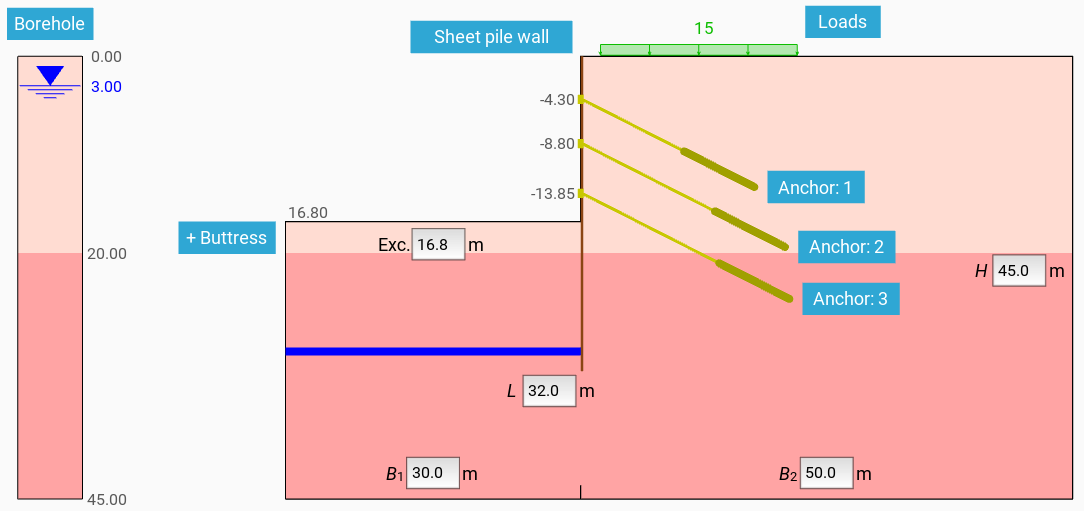
\includegraphics[width=\textwidth]{images/zswalls_setup.png}
	\caption{\texttt{ZSWalls} basic configuration. Consider top soil as elastic, we want to deduce Young modulus $E$ from displacement $U_x$.}
	\end{figure}
	\end{frame}
	
	\begin{frame}{\texttt{ZSWalls} setup: deep excavation}
	\begin{columns}
	\begin{column}{.5\textwidth}
	\begin{block}{Displacement model $U_x(E)$}
	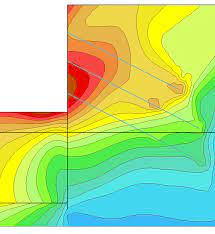
\includegraphics[width=\textwidth]{images/settlement.jpg}
	\end{block}
	\end{column}
	\begin{column}{.5\textwidth}
	\begin{block}{Setup}
	\begin{itemize}
	\item Prior: $E_{prior} = 10000 \si{KPa}$, COV $20\%$.
	\item Correlation length: $l_x = 5\si{m}$, $l_y = 1\si{m}$.
	\item Measurements: $2 \si{cm}$, error $10\%$, taken at the top-left corner.
	\end{itemize}
	\end{block}
	\end{column}
	\end{columns}
	\end{frame}
	
	\begin{frame}{Posterior mean of Young modulus}
	\begin{figure}
	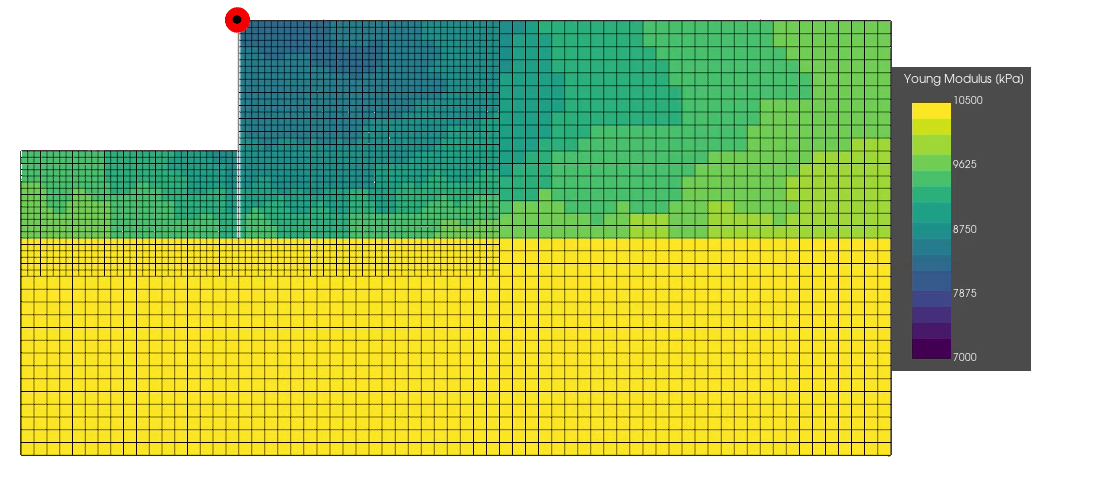
\includegraphics[width=\textwidth]{graphs/final/mean_rf_Eprior=10000_gimped.png}
	\caption{Mean of $E_{post}$ in finite element visualization. Measurement point highlighted in red in the top-left corner.}
	\end{figure}
	\end{frame}
	
	\begin{frame}{Posterior standard deviation of Young modulus}
	\begin{figure}
	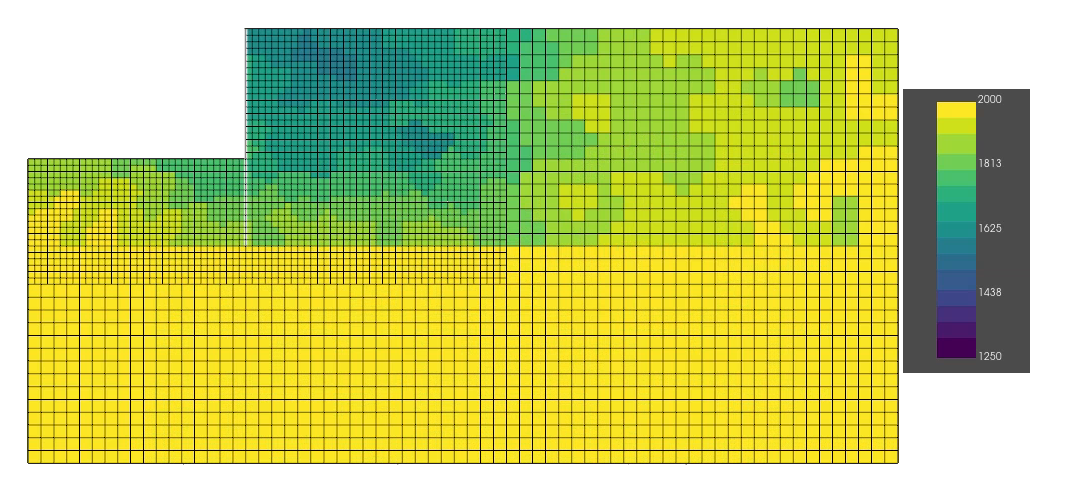
\includegraphics[width=\textwidth]{graphs/final/std_rf_Eprior_std=2000_gimped.png}
	\caption{Standard deviation of $E_{post}$ in finite element visualization, varying from $1250 \si{KPa}$ to $2000 \si{KPa}$. }
	\end{figure}
	\end{frame}
	
	\begin{frame}{Conclusions}
	\begin{columns}
	\begin{column}{.5\textwidth}
    \begin{block}{Reliability of the method}
    It depends on:
    \begin{itemize}
	\item Where the measurements are taken.
	\item How correlation was estimated.
	\item How discrepancy was estimated.
	\end{itemize}
	\end{block}
	\end{column}
	\begin{column}{.5\textwidth}
	\begin{block}{Interpret uncertainty}
	\begin{itemize}
	\item Good estimation: must be smaller than the prior.
	\item Solution sensitivity.
	\item Accuracy on approximations (model, methods, ...).
	\end{itemize}
	\end{block}
	\end{column}
	\end{columns}
	\end{frame}
	
	%----------------------------------------------
	%\section{Bibliography}
		
	%	\begin{frame}[allowframebreaks]
			
	%		\tiny\bibliographystyle{apalike}
	%		\bibliography{ref}	
			
			 %\tiny\bibliographystyle{alpha}
            
	%	\end{frame}

	%-------------------------------------------
    \begin{frame}
	    \begin{center}
		{\Huge \emph {\textrm{Thank  ~you!}}}
		\end{center}
    \end{frame}

\end{document}